\section{实验验证与分析}

\subsection{数据集和指标}
本章方法在YCB-V数据集\cite{ycbv}和IC-BIN数据集\cite{icbin}上进行了验证,遵循BOP挑战赛\cite{hodan2024bop}的设置和评估指标。训练阶段使用了50,000张仿真合成图像,而测试阶段则在真实图像上进行。评估采用了三个指标:可见表面差异(VSD)、最大对称感知表面距离(MSSD)和最大对称感知投影距离(MSPD)。这三个指标的平均值(记为AR)被用作整体性能的衡量标准。关于评价指标的详细内容参照\autoref{subsec:评价指标}。

\subsection{与现有方法的比较}

\textbf{在YCB-V数据集上的BOP指标对比 } 该方法与其他完全在合成数据上训练的方法在YCB-V数据集上的表现进行了比较,结果如\autoref{tab:ca_ycbv_bop}所示。术语“PBR”表示模型完全在合成图像上训练,而“RGB”表示输入中未使用深度信息。向上箭头(↑)表示较高的指标值代表更好的性能,而向下箭头(↓)则相反。采用了BOP挑战赛2023\cite{hodan2024bop}提供的默认检测结果。实验结果表明,提出的方法在仅需0.019秒的运行时间下,能够将基线方法的性能提升。具体而言,该方法比上一章模型SymNet\cite{symnet}提高了$0.9\%$,并且在不使用深度信息的情况下,达到了接近使用RGB-D图像作为输入的FFB6D\cite{he2021ffb6d}的准确性。与其他需要渲染优化的技术相比,该方法在运行时间上仍具有显著优势。

\begin{table}[ht]
        \centering
        \caption{
                YCB-V数据集上的BOP评估结果
        }
        \resizebox{\textwidth}{!}{%
        \begin{tabular}{l c c c c c c c c}
        \toprule
        6D 物体位姿估计方法 & 输入类型 & 训练类型&$AR\uparrow$&$AR_{VSD}\uparrow$&$AR_{MSSD}\uparrow$&$AR_{MSPD}\uparrow$&时间(s)$\downarrow$\\       %表格第一行,&的位置对齐
        \midrule
        CDPNv2~\cite{li2019cdpn}&RGB&PBR&53.2&39.6&57.0&63.1&0.143 \\
        CosyPose~\cite{labbe2020cosypose}&RGB&PBR&57.4&51.6&55.4&65.3&0.342\\
        EPOS~\cite{hodan2020epos}&RGB&PBR&49.9&41.1&46.4&62.1&0.764 \\
        SurfEmb~\cite{haugaard2022surfemb}&RGB&PBR&64.7&54.8&62.0&77.3&5.427 \\
        GDRNPP~\cite{wang2021gdr}&RGB&PBR&71.3&59.9&70.8&\textbf{83.1}&0.277\\
        ZebraPoseSAT-EffnetB4~\cite{su2022zebrapose}&RGB&PBR&72.9&64.0&72.5&82.1&0.25 \\
        SymNet~\cite{symnet}&RGB&PBR&73.9&63.8&75.1&82.6&\textbf{0.091} \\
        Contour Alignment(本章)&RGB&PBR&\textbf{74.8}&\textbf{66.0}&\textbf{75.3}&\textbf{83.1}&0.110\\
        \midrule
        CDPNv2+ICP~\cite{li2019cdpn}&RGB-D&PBR+real&61.9&59.0&70.1&56.5&0.637\\
        Pix2Pose+ICP~\cite{park2019pix2pose}&RG-D&PBR+real&67.5&69.3&70.3&63.0&2.106\\
        \midrule
        FFB6D~\cite{he2021ffb6d}&RGB-D&PBR&75.1&70.6&82.7&74.0&0.199\\
        \bottomrule
        \end{tabular}
        }
\label{tab:ca_ycbv_bop}
\end{table}


\textbf{在IC-BIN数据集BOP指标对比}

将本章方法与完全在合成数据上训练的其他方法进行比较在IC-BIN数据集上,如\autoref{tab:ca_icbin_bop}所示。术语“PBR”表示模型完全在合成图像上训练,而“RGB”表示输入中未使用深度信息。向上箭头(↑)表示较高的指标值表示更好的性能,而向下箭头(↓)表示相反。采用BOP挑战赛2023\cite{hodan2024bop}提供的默认检测结果。与其他方法相比,该方法运行时间显著减少,因为细化方法不依赖于另一个耗时的网络。该方法在准确性和运行时间方面都取得了优异的结果。在该数据集的实验上,该方法对基线方法没有显著提升,这也说明了该方法的局限性。但综合在YCB-V以及在IC-BIN的结果,说明了该方法总体上是有效果的。

\begin{table}[htbp]
        \centering
        \caption{
                IC-BIN 数据集上的 BOP 评估结果
        }
        \resizebox{\textwidth}{!}{%
        \begin{tabular}{l c c c c c c c c}
        \toprule
        6D 物体位姿估计方法 &输入类型&训练类型&$AR\uparrow$&$AR_{VSD}\uparrow$&$AR_{MSSD}\uparrow$&$AR_{MSPD}\uparrow$&时间 (s)$\downarrow$\\
        \midrule
        CRT-6D~\cite{castro2023crt}&RGB&pbr&53.7&\textbf{47.7}&51.7&61.8&0.120 \\
        ZebraPoseSAT-EffnetB4&RGB&pbr&54.5&47.5&\textbf{53.5}&62.5&0.25 \\
        SymNet&RGB&pbr&\textbf{54.7}&45.0&51.1&\textbf{67.8}&\textbf{0.088} \\
        Contour Alignment(本章)&RGB&pbr&\textbf{54.7}&45.4&51.1&67.7&0.098 \\
        \bottomrule
        \end{tabular}
        }
\label{tab:ca_icbin_bop}
\end{table}

\subsection{消融实验}

本节通过多项的消融研究,探讨多种因素对该方法性能的影响,包括Tikhonov正则化、优化过程的停止条件以及迭代次数。所有实验均在YCB-V数据集上进行,并采用平均召回率(AR)作为性能评估指标。

\textbf{Tikhonov参数的作用 } 如\autoref{tab:ca_main_ablation}所示,对比了不使用优化过程以及使用优化的结果。实验表明,如果不使用Tikhonov正则化,则AR会直接下降4.1\%。缺乏Tikhonov正则化会导致准确性下降,突出了Tikhonov正则化在优化稳定性中的关键作用。使用了Tikhonov正则化后,平均召回率提升0.9\%。通过对运行时间的测试,可以得出Tikhonov正则化不会对运行时间产生太大的影响。

\begin{table}[ht]
  \centering
  \caption{关于优化和 Tikhonov 正则化的消融研究}
  \begin{tabular}{@{}c|c|c|c@{}}
    \toprule
    使用优化 & Tikhonov 正则化 & $AR\uparrow$ & 运行时间 (秒) \\
    \midrule
               &                         & 73.9         & 0.091      \\
    \checkmark &                         & 69.8         & 0.110      \\
    \checkmark & \checkmark              & 74.8         & 0.111      \\
    \bottomrule
  \end{tabular}
  \label{tab:ca_main_ablation}
\end{table}


  %   A0 & w early stop (ours) & 74.8 & 0.110\\
  %   B0 & w/o Tikhonov regularization & 73.9 & 0.091 \\
  %   C0 & w/o refinement & 73.9 & 0.091 \\
  %   \midrule
  %    Tikhonov parameter = $10^1$ & 74.8 & 0.109 \\
  %    Tikhonov parameter = $10^2$ & 74.8 & 0.108 \\
  %    Tikhonov parameter = $10^3$ & 74.8 & 0.110 \\
  %    Tikhonov parameter = $10^4$ & 74.8 & 0.110 \\
  %    Tikhonov parameter = $10^5$ & 74.9 & 0.112 \\
  %    Tikhonov parameter = $10^6$ & 75.1 & 0.113 \\
  %    Tikhonov parameter = $10^7$ & 75.1 & 0.110 \\
  %    Tikhonov parameter = $10^8$ & 74.9 & 0.112 \\
  %    Tikhonov parameter = $10^9$ & 74.1 & 0.109 \\
  %   \bottomrule
  % \end{tabular}
%   \label{tab:Tikhonov}
% \end{table}
% \begin{table}
%   \centering
%     \caption{The influence of iteration step}
%   \begin{tabular}{@{}c|c|c@{}}
%     \toprule
%     settings & $AR\uparrow$ & time (sec) \\
%     \midrule
%      w/o refinement & 73.9 & 0.091 \\
%      \midrule
%      iteration step = $1$ & 74.7 &  0.100\\
%      iteration step = $2$ & 74.7 &  0.103\\
%      iteration step = $3$ & 74.8 &  0.106\\
%      iteration step = $4$ & 74.8 &  0.108\\
%      iteration step = $5$ & 74.8 &  0.109\\
%      iteration step = $6$ & 74.8 &  0.110\\
%      iteration step = $7$ & 74.8 &  0.111\\
%      \midrule
%      w early stop (ours) & 74.8 & 0.110\\
%     \bottomrule
%   \end{tabular}
%   \label{tab:ablation_iter}
% \end{table}


\textbf{Tikhonov参数鲁棒性 } 此外,验证了Tikhonov参数的鲁棒性,\autoref{tab:ca_Tikhonov_Parameter}展示了Tikhonov参数$\lambda$在$10$到$10^8$范围内以10的幂次为间隔的满意性能。与\autoref{tab:ca_main_ablation}中使用优化而不使用Tikhonov正则化的结果$AR=69.8\%$相比,使用Tikhonov正则化可以明显带来正收益。当Tikhonov参数$\lambda$小于$10^5$时结果$AR$可达到$74.8\%$,当$\lambda=10^6$,算法精度达到最高75.1,并且只有当$\lambda>=10^9$才能够观测到AR的明显下降。实验表明Tikhonov参数的鲁棒性极强,在10至$10^8$均为合理范围。推荐使用$\lambda=10^6$作为默认参数。

\begin{table}[ht]
  \centering
  \caption{Tikhonov 参数的影响}
  \begin{tabular}{c|c|c|c|c|c|c|c|c|c}
    \toprule
    $\lambda$ & $10$ & $10^2$ & $10^3$ & $10^4$ & $10^5$ & $10^6$ & $10^7$ & $10^8$ & $10^9$ \\
    \midrule
    AR & 74.8 & 74.8 & 74.8 & 74.8 & 74.9 & 75.1 & 75.1 & 74.9 & 74.1 \\
    \bottomrule
  \end{tabular}
  \label{tab:ca_Tikhonov_Parameter}
\end{table}

  %    Tikhonov parameter = $10^1$ & 74.8 & 0.109 \\
  %    Tikhonov parameter = $10^2$ & 74.8 & 0.108 \\
  %    Tikhonov parameter = $10^3$ & 74.8 & 0.110 \\
  %    Tikhonov parameter = $10^4$ & 74.8 & 0.110 \\
  %    Tikhonov parameter = $10^5$ & 74.9 & 0.112 \\
  %    Tikhonov parameter = $10^6$ & 75.1 & 0.113 \\
  %    Tikhonov parameter = $10^7$ & 75.1 & 0.110 \\
  %    Tikhonov parameter = $10^8$ & 74.9 & 0.112 \\
  %    Tikhonov parameter = $10^9$ & 74.1 & 0.109 \\

\textbf{迭代步骤 } 通过评估每次迭代的平均召回率(AR),展示了该方法的收敛性,如\autoref{tab:ca_Iteration_Step}所示。可以观察到,第一次迭代步骤对整体改进贡献显著,AR从73.9提升至74.7。随后几次迭代的改进逐渐减小,最终在第4次迭代后趋于稳定。此外,自动停止条件能够在不需要手动确定迭代次数的情况下实现与固定迭代次数相同的最佳结果(AR=74.8)。

\begin{table}[ht]
  \centering
  \caption{Influence of Iteration Step}
  \scalebox{1.0}{
  \begin{tabular}{c|c|c|c|c|c|c}
    \toprule
    $\lambda$ & w/o & 1 & 2 & 3,4,5,6,7,8 & 9 & early stopping \\
    \midrule
    AR & 73.9 & 74.7 & 74.7 &74.8 & 74.8 &74.8 \\
    \bottomrule
  \end{tabular}
  }
  \vspace{-0.2cm}
  \label{tab:Iteration Step}
\end{table}


\subsection{运行时间分析}

该方法通过避免复杂的网络细化,并结合自动停止策略,有效减少了计算开销。在高速端到端的SymNet网络中集成后,本章的优化方法在运行时间上展现出显著优势。整体执行时间(包括渲染和优化)仅为0.02秒,显著优于其他主流方法。

\subsection{可视化}
\par \textbf{训练数据和测试数据 } 该方法在仿真数据上进行了训练,仿真数据中包含了无关物体,并模拟了各种背景、光照条件以及遮挡情况。左图展示了在50,000张合成图像上进行训练的场景。右图(第一行)为来自真实场景的测试图像,右图(第二行)为使用恢复的姿态在场景中渲染的物体模型。由于在训练中使用了足够强的数据增广,能够有效完成跨域任务。合成训练集和真实测试集及其对应真值标签可视化见\autoref{fig:ca_quantitative_results}。

\begin{figure}[htbp]
    \centering
    \begin{overpic}[width=1.0\textwidth]{figure/ca/main_explain_paper.jpg}
        \put (10, 31) {\textbf{\textcolor{white}{在合成图像上训练}}}
        \put (60, 31) {\textbf{\textcolor{white}{在真实图像上推理}}}
    \end{overpic}
    \caption{结果可视化}
    \label{fig:ca_quantitative_results}
\end{figure}




\textbf{细节展示 } 在\autoref{fig: ca_detail_compare}中强调了优化过程的作用。展示了SymNet\cite{symnet}(在明亮的蓝色背景中显示)和该方法(在明亮的绿色背景中显示)之间的视觉比较,突出了细化过程的影响,展示了其有效性。SymNet端到端网络的输出边缘与实物有些许偏差的情况下,该方法能够对此进行优化。将估计的位姿渲染回原始图像,并观察到细化后的渲染结果与原始图像的一致性更高。

\begin{figure}[htbp]
\centerline{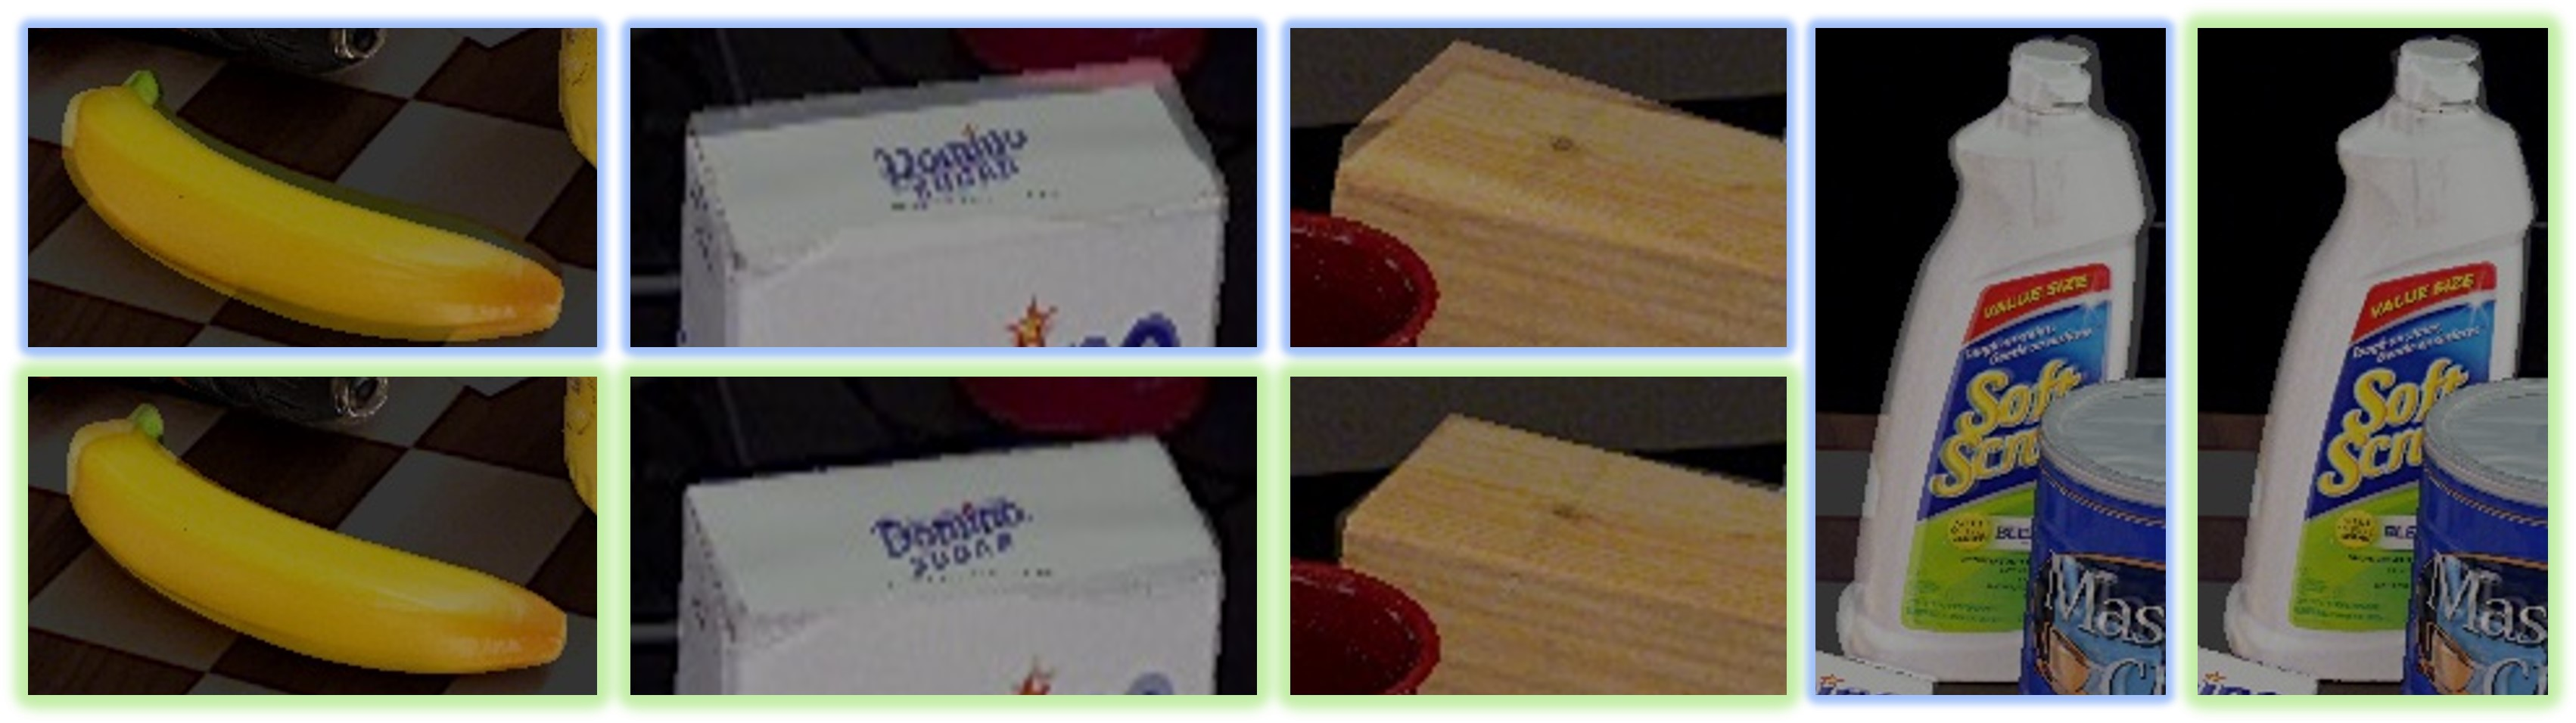
\includegraphics[width=1.0\textwidth]{figure/ca/detail_compare.jpg}}
    \caption{细节展示}
    \label{fig: ca_detail_compare}
\end{figure}

\textbf{工作原理展示 } \autoref{fig:optimization_vis}展示了对齐前后CoI、$\bm{C}_\text{ren}$和$e_i$的可视化效果。左图为RGB图像,中间和右图分别展示了对齐前后的CoI、$\bm{C}_\text{ren}$和$e_i$。为了更清晰地呈现,$e_i$以稀疏形式绘制。文本颜色与对应的视觉元素颜色保持一致,以便于理解。

\begin{figure}[thbp]
    \centering
    \begin{overpic}[width=1.0\textwidth]{figure/ca/optimization_vis.jpg}
        \put (35,4) {\textcolor{red}{$e = 2.69$}}
        \put (69,4) {\textcolor{red}{$e = 0.64$}}
        \put (39,25) {\textcolor{black}{CoI}}
        \put (73,25) {\textcolor{black}{CoI}}
        \put (52,18) {\textcolor{cyan}{$\bm{C}_\text{ren}$}}
        \put (85,18) {\textcolor{cyan}{$\bm{C}_\text{ren}$}}
    \end{overpic}
    \caption{轮廓对齐}
    \label{fig:optimization_vis}
\end{figure}

\begin{figure}[htbp]
    \centerline{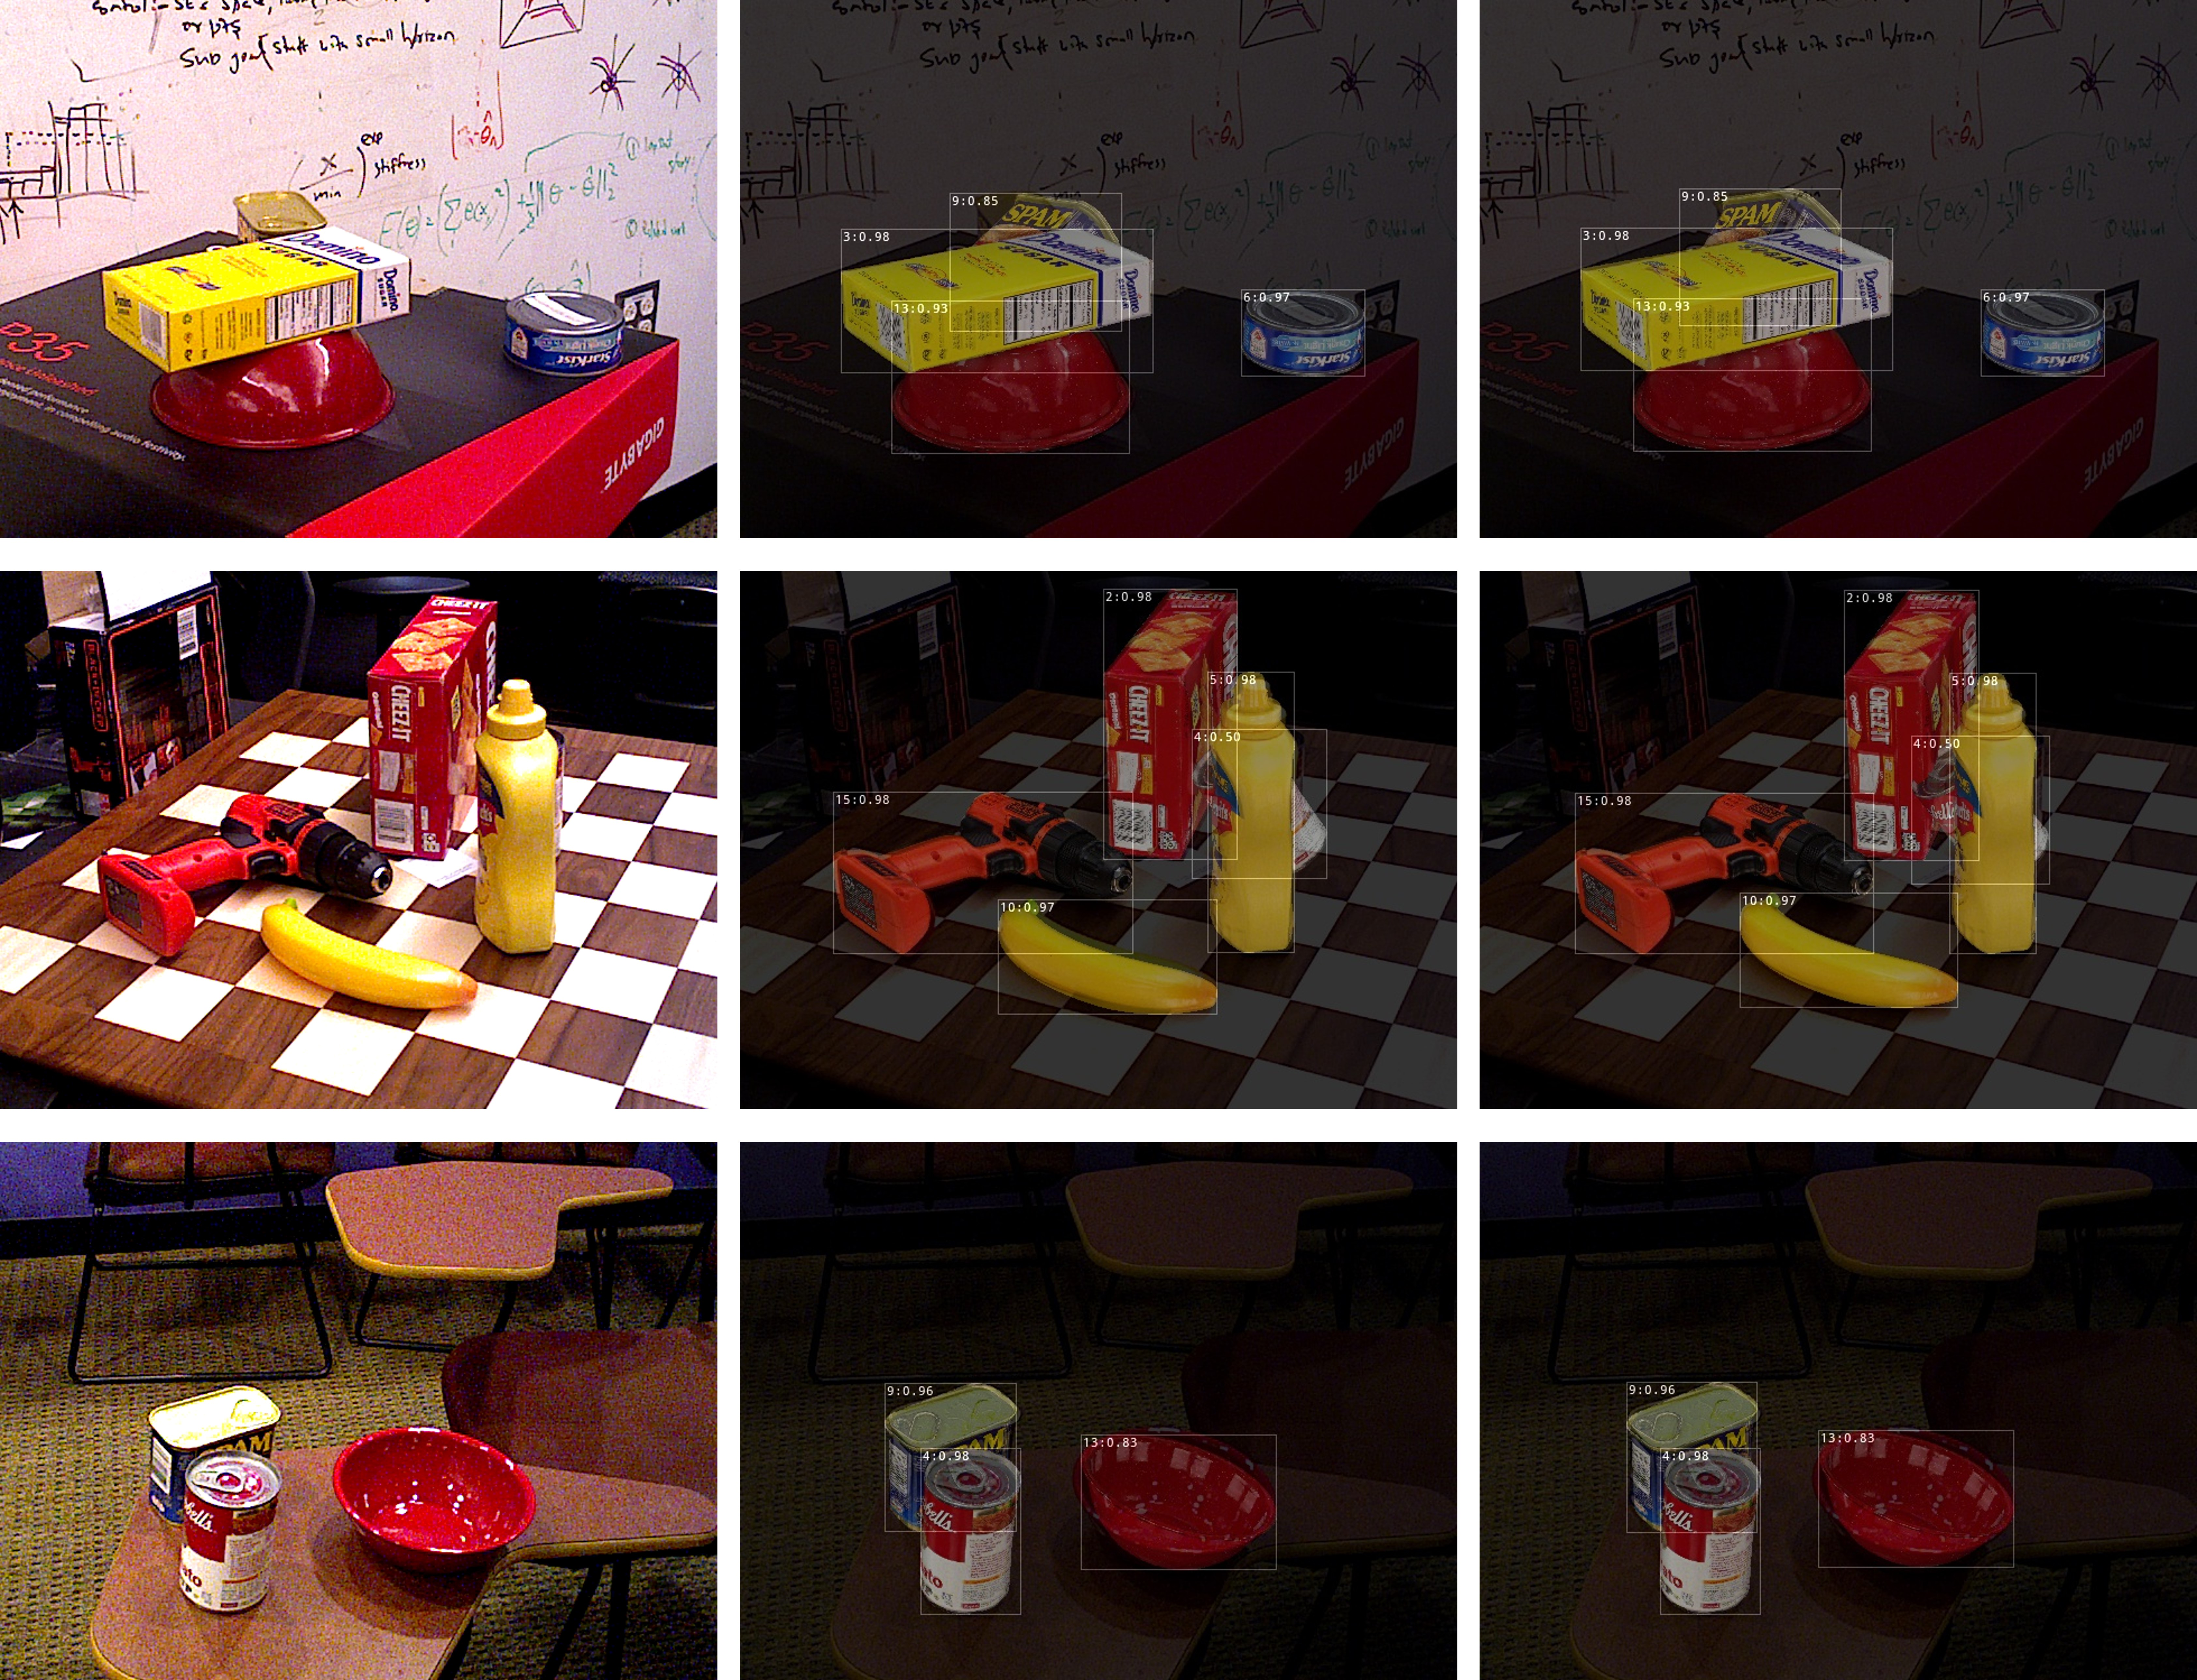
\includegraphics[width=1.0\textwidth]{figure/ca/failure_case.jpg}}
        \caption{失败案例分析}
        \label{fig: failure_case}
\end{figure}

\textbf{失败案例分析 } 在\autoref{fig: failure_case}中展示了一些失败案例。最左列为RGB图像,中间列为SymNet的预测结果,最右列为经过优化后的结果。从图中可以看出,大多数失败案例集中在物体被严重遮挡的情况下。这些失败的主要原因是初始位姿估计存在较大的误差。值得注意的是,没有发现优化过程导致结果显著恶化的情况。这表明,尽管本文提出的细化方法在优化初始估计方面表现良好,但对于初始误差较大的情况,其效果仍然有限,这也反映了方法的局限性。